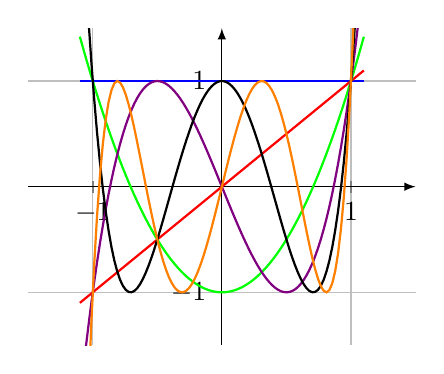
\begin{tikzpicture}
    \begin{axis}[width=6.5cm,
        axis lines=middle,
        inner axis line style={-latex},
        grid=major,
        xmin=-1.5, xmax=1.5,
        ymin=-1.5, ymax=1.5,
        % xlabel=$x$, xlabel style={right},
        % ylabel=$y$, ylabel style={above},
        tick style={thick},
        ticklabel style={font=\normalsize},
        xtick={-1, 0, 1}, 
        ytick={-1, 0, 1},
        % legend entries={0.5x},
            legend style={
            at={(1.05,0.4)},
            anchor=north,
            legend columns=1},
            legend cell align={left}
    ]
    
    \def\a{-1.1}
    \def\b{1.1}
    
    \addplot[blue,thick,samples=100,domain=\a:\b] {1};
    \addplot[red,thick,samples=100,domain=\a:\b] {x};
    \addplot[green,thick,samples=100,domain=\a:\b] {2*x^2-1};
    \addplot[violet,thick,samples=100,domain=\a:\b] {4*x^3-3*x};
    \addplot[black,thick,samples=100,domain=\a:\b] {8*x^4-8*x^2+1};
    \addplot[orange,thick,samples=100,domain=\a:\b] {16*x^5-20*x^3+5*x};
    
   % \legend{$\Leg_0$, 
   %         $\Leg_1$,
%            $\Leg_2$,
%            $\Leg_3$,
 %           $\Leg_4$,
  %          $\Leg_5$
   %         }
    \end{axis}
\end{tikzpicture}